\documentclass[a4paper,12pt]{article}
\usepackage[utf8]{inputenc}
\usepackage[cm,empty]{fullpage}
\usepackage[T2A]{fontenc}
\usepackage[english, russian]{babel}
\usepackage{amssymb,amsmath,amsxtra,amsthm}
\usepackage{proof}
\usepackage[pdftex]{graphicx}
\usepackage{wrapfig}
\usepackage{xcolor}


\usepackage[left=2cm,right=2cm,
    top=1cm,bottom=1cm,bindingoffset=0cm]{geometry}

\renewcommand{\leq}{\leqslant}
\renewcommand{\geq}{\geqslant}


\newcommand{\iiff}{\Longleftrightarrow}
\renewcommand{\iff}{\Leftrightarrow}
\newcommand{\nothing}{\varnothing}


\newcommand{\NN}{\mathbb{N}}
\newcommand{\ZZ}{\mathbb{Z}}
\newcommand{\Q}{\mathbb{Q}}
\newcommand{\A}{\mathbb{A}}
\newcommand{\R}{\mathbb{R}}
\renewcommand{\C}{\mathbb{C}}

\renewcommand{\phi}{\varphi}
\newcommand{\eps}{\varepsilon}

\newcounter{z}


\newcommand{\zs}{\refstepcounter{z}\vskip 10pt\par\noindent
\fbox{\textbf{12.\arabic{z}}} }

\newcommand{\z}{\refstepcounter{z}\vskip 20pt\noindent
\fbox{\textbf{\arabic{z}}} }

\renewcommand{\date}{{\bf 21 января 2020}} %Дата занятия

\newcommand{\dif}
{
------------------------------------------------------------------------------------------------------------------------------------------------------
}

\newcommand{\HSEhat}{



{\bf \phantom{\date}  \large \hfill Дискретная математика: \hfill \normalsize \date}

\vspace{5 pt}
{\bf \large \hfill  комбинаторика и вероятность.\hfill }

\vspace{15 pt}
\centerline{ \large  Домашнее задание №2.}

\vspace{15 pt}
\centerline{ \large  Кирилл Сетдеков}


\vspace*{10pt}
\setcounter{z}{0}

}

\begin{document}

\HSEhat

\z После опроса $250$ человек оказалось, что английский знают ровно $210$ респондентов, испанский --- $100$, а оба языка --- $80$. Сколько из опрошенных не знают ни английского, ни испанского?

\begin{wrapfigure}{r}{0.4\textwidth} 
    \centering
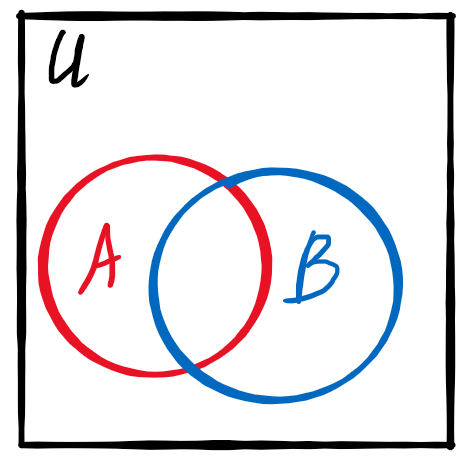
\includegraphics[scale=1]{ab.png}
\end{wrapfigure}
\textbf{Решение:} 

Пусть $U$ - все участвовавшие в опросе люди, тогда:
$$|U| = 250; |A| = 210; |B| = 100; |A \cap B| = 80$$
Нас интересует $|U\backslash(A \cup B)|$

$$|A \cup B| = |A| + |B| - |A \cap B| = 210+100-80=230$$
$$|U\backslash(A \cup B)| = |U| - |A \cup B| = 250-230=20$$

\textbf{Ответ: 20}

\z Есть $10$ кандидатов на $6$ различных вакансий. Каждого кандидата можно взять на любую вакансию. Сколькими способами можно заполнить вакансии? (Каждая вакансия должна быть заполнена ровно одним человеком.

\textbf{Решение:} \\
Нас интересует количество размещение из 10 по 6, так как нам важно, какой из 6 человек занимает какую вакансию. 
$$A^6_{10} = \frac{10!}{4!} = 151200$$

\textbf{Ответ: 151200}

\z Найдите вероятность того, что в случайном шестизначном коде будет хотя бы две одинаковые цифры.

\textbf{Решение:}\\
В шестизначном коде $10^6$ вариантов. Чтобы у нас все цифры были разные, необходимо выбрать 6 уникальных цифр из 10, таких способов $A^6_{10}$.

Тогда, если считать событие <<В коде есть хотя бы 2 одинаковые цифры>> = $A$, <<В коде все цифры уникальные>> = $A^c$,
$|\Omega| = 10^6$
$$P(A^c) = \frac{|A^c|}{|\Omega|}=\frac{A^6_{10}}{10^6}=\frac{151200}{10^6}$$
$$P(A) = 1-P(A^c) = 1- \frac{A^6_{10}}{10^6}= \frac{1061}{1250}\approx0.8488$$



\textbf{Ответ: $\frac{1061}{1250}\approx0.8488$}

\z {\bf a)} Каких натуральных чисел больше среди первого миллиона: тех, в записи которых
есть единица или тех, в записи которых её нет?

\textbf{Решение:}\\
Пусть событие <<Есть хотя бы 1 единица в записи>> = $A$, тогда $A^c$ =  <<В записи числа нет ни 1 единицы>>. Нам нужно сравнить ${P(A)} vs {P(A^c)}$. Все возможные числа до 1 миллиона - $\Omega$.
$$|\Omega| = 10^6$$ так как мы можем выбрать любую цифру для каждого из 6 знаков.
$$|A^c| = 9^6$$ так как если взять в любом разряде цифру кроме 1, то остается 9 цифр и получится число без единиц.
$$P(A^c) = \frac{|A^c|}{|\Omega|}=\frac{9^6}{10^6}\approx0.5314$$
$$P(A) = 1-P(A^c)=1- \frac{|A^c|}{|\Omega|}=\frac{10^6-9^6}{10^6}\approx0.4686$$
$$P(A^c) > P(A)$$

\textbf{Ответ: Чисел где нет ни одной единицы больше чем чисел где есть хотя бы одна единица, среди чисел до 1 миллиона}

{\bf б)} Тот же вопрос для первых 10 миллионов чисел.

(В нашем курсе мы считаем, что натуральные числа начинаются с $0$.)

\textbf{Решение:}\\
Аналогично, <<Есть хотя бы 1 единица в записи>> = $A$, тогда $A^c$ =  <<В записи числа нет ни 1 единицы>>. Нам нужно сравнить ${P(A)} vs {P(A^c)}$. 

Все возможные числа до 10 миллиона - $\Omega$.
$|\Omega| = 10^7$ так как мы можем выбрать любую цифру для каждого из 7 знаков и $|A^c| = 9^7$.
$$P(A^c) = \frac{|A^c|}{|\Omega|}=\frac{9^7}{10^7}\approx0.4783$$
$$P(A) = 1-P(A^c)=1- \frac{|A^c|}{|\Omega|}=\frac{10^7-9^7}{10^7}\approx0.5217$$
$$P(A^c) < P(A)$$

\textbf{Ответ: Чисел где есть хотя бы одна единица больше чем чисел где нет ни одной единицы, среди чисел до 10 миллионов}
\z Найдите вероятность выпадения дубля при броске двух кубиков (дубль означает, что на обоих кубиках выпало одинаковое значение).

\textbf{Решение:}\\
Пусть событие <<Выпал дубль из двух кубиков>> = $A$, все возможные броски двух кубиков - $\Omega$.

Перечислим все возможные исходы, которые мы считаем дублями как значения на каждом кубике. Событие $A$ будет множеством элементарных событий $$A= \{{(1,1), (2,2), (3,3), (4,4), (5,5), (6,6)}\}$$
$$|A| = 6;|\Omega|=36; P(A) = \frac{|A|}{|\Omega|}=\frac{6}{36}= \frac{1}{6}$$

\textbf{Ответ: $\frac{1}{6}$}
\z Команда принимает участие в турнире, где сыграет {\it четыре} игры.

Вероятность выиграть в первом матче равна $\frac 12$. Вероятность выигрыша после победы в предыдущем матче возрастает до $\frac 23$, а после поражения уменьшается до $\frac 13$.

Нарисуем дерево решений:

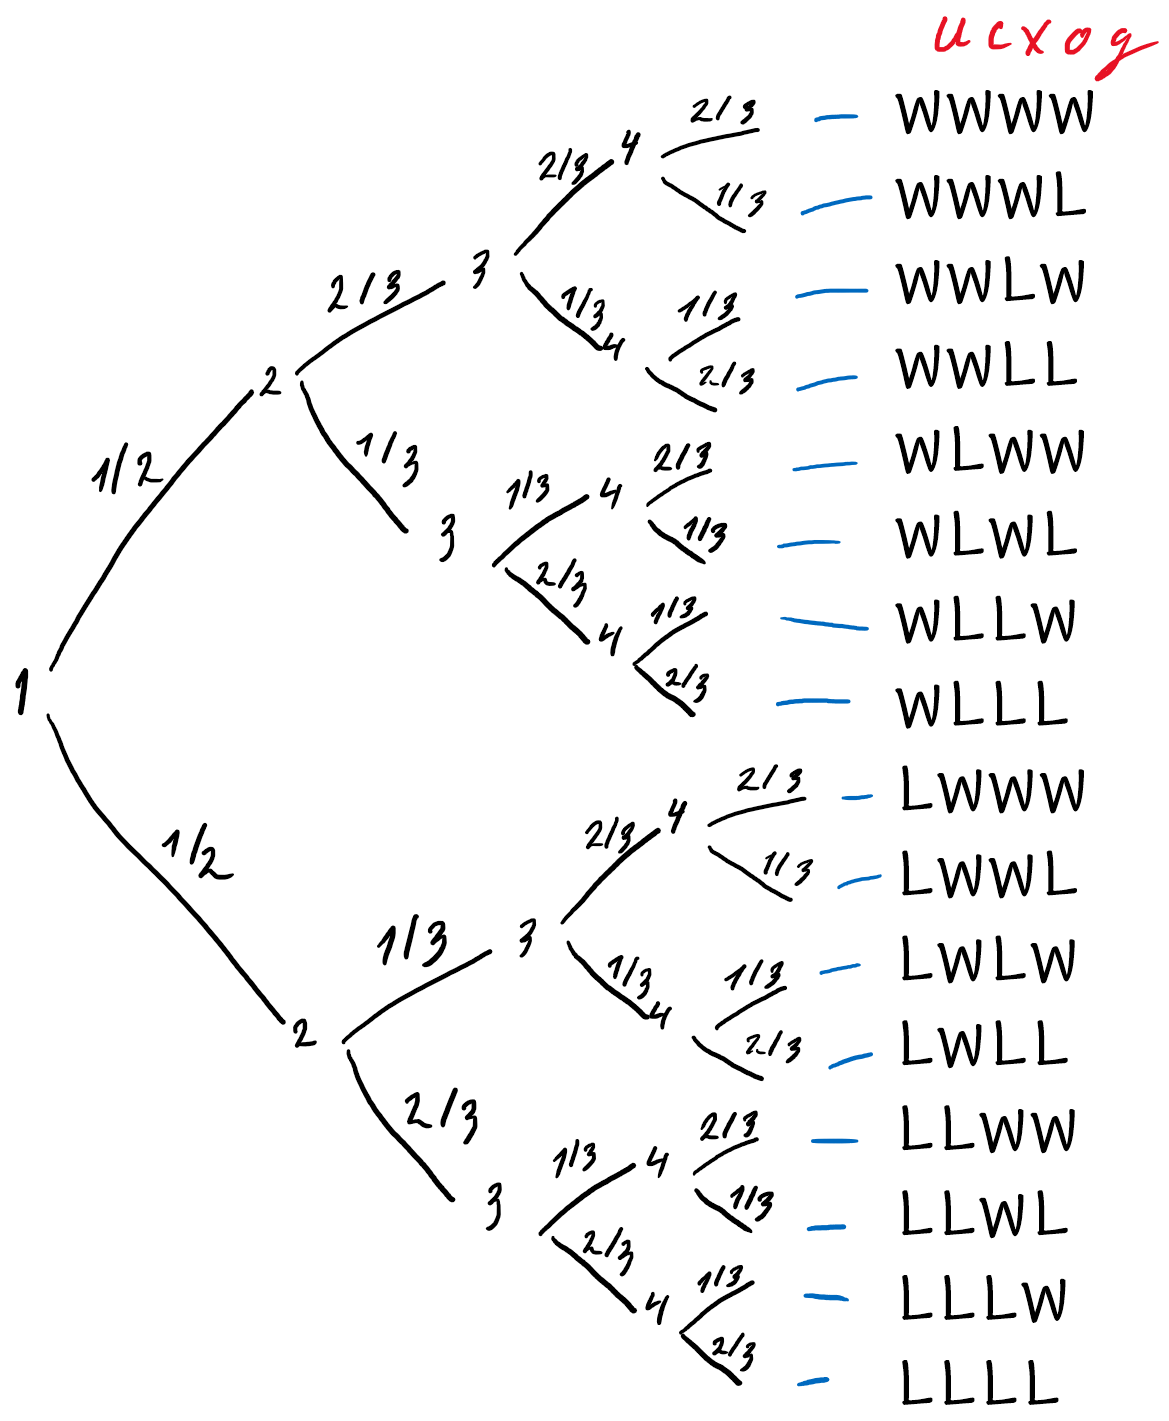
\includegraphics[scale=1]{tree.png}


Какова вероятность

{\bf a)} выиграть не менее двух игр?

\textbf{Решение:}\\
Пусть $X$ - число выигранных игр. Нас интересует $P(X\geq2)$.
$$P(X\geq2) = 1 - P(X<2) = 1 - P(X = 0) - P(X = 1)$$
Выиграть 0 игр можно 1 способом - проиграть все, т.е. получить следующую последовательность выигрышей: $(L, L, L, L)$, где $W$ - выигрыш и $L$ проигрыш. Вероятность этого события равна произведению вероятностей каждого из последовательных исходов матчей. Возьмем их из дерева.
$$P(X = 0) = P(L, L, L, L) =\frac{1}{2}\times\frac{2}{3}\times\frac{2}{3}\times\frac{2}{3} = \frac{4}{27}$$
Для числа выигрышей = 1, есть 4 варианта:
$$(W, L, L, L), (L, W, L, L), (L, L, W, L), (L, L, L, W)$$
Выпишем для них вероятности из дерева решений
$$
P(X = 1) = P(W, L, L, L)+P(L, W, L, L) + P(L, L, W, L)+P(L, L, L, W) \\= \frac{2}{27}+\frac{1}{27}+\frac{1}{27}+\frac{2}{27} = \frac{6}{27}
$$
Запишем ответ:
$$P(X\geq2) = 1 - \frac{4}{27} - \frac{6}{27} = \frac{17}{27} \approx0.6296$$

\textbf{Ответ: $\frac{17}{27} \approx0.6296$}

{\bf б)} выиграть ровно две игры?

\textbf{Решение:}\\
Из 4 игры будет 6 возможных последовательностей игр, где выиграно ровно 2. $C^2_4 = 6$. Эти последовательности: 
$$(W, W, L, L), (W, L, W, L), (W, L, L, W), (L, W, W, L), (L, W, L, W), (L, L, W, W)$$
$$P(X = 2) =  \frac{2}{27}+\frac{1}{54}+\frac{1}{27}+\frac{1}{27}+\frac{1}{54}+\frac{2}{27} = \frac{7}{27}\approx0.259$$

\textbf{Ответ: $\frac{7}{27} \approx0.259$}

\z Монету бросают восемь раз. Найдите вероятности событий:

{\bf a)} $A$ --- "орел выпал 6 раз";

\textbf{Решение:}\\
Считаем, что это это испытание Бернулли, где $p=1/2; N=8, k=6$. Тогда вероятность события A:
$$P(A) = C^k_N\times p^k \times (1-p)^{N-k} = C^6_8\times ({\frac{1}{2}})^6 \times ({\frac{1}{2}})^{2} = C^6_8\times ({\frac{1}{2}})^8= \frac{28}{2^8}=\frac{7}{64}$$

\textbf{Ответ: $\frac{7}{64} \approx0.109$}

{\bf б)} $B$ --- "орел выпал не менее трех раз".

\textbf{Решение:}\\
X - число выпавших орлов.
$$P(B) = P(X \geq 3)=1-P(B^c)= 1-P(X<3)$$
$P(A)$ уже известно и $P(A) = P(X=6) = P(X=2)$ так как $C^6_8=C^2_8$. Также $P(X<3) = P(X=0)+P(X=1)+P(X=2)$. Можно выразить:
$$P(B) = 1-P(X=0)-P(X=1)-P(A)$$
Осталось посчитать $P(X=0)$ и $P(X=1)$.
$$P(X=0) = C^0_8\times ({\frac{1}{2}})^8= \frac{1}{2^8}$$
$$P(X=1) = C^1_8\times ({\frac{1}{2}})^8= \frac{8}{2^8}$$


$$P(B) = 1-\frac{1}{2^8}-\frac{8}{2^8}-\frac{28}{2^8} =\frac{219}{256} $$

\textbf{Ответ: $\frac{219}{256} \approx0.855$}

\end{document}

